\section{Modelos}
\begin{frame}
% \blfootnote{\footcite{aggarwal_recommender_2016}}
\begin{itemize}
    \item<1-> \textbf{Basado en contenido}\onslide<3->{: PLN del texto de las propuestas}
    \item<2-> \textbf{Basado en filtrado colaborativo}\onslide<3->{: Graph Neural Networks (LightGCN)}
    \item<4-> \textbf{Híbrido}: Ensamblaje de los dos anteriores
    % \item<5-> \color{gray}{\textbf{Basado en conocimiento}: No hecho\footnote{\footcite{valiente_integration_2022}}}
\end{itemize}
\end{frame}

\subsection{Modelo basado en contenido}
\begin{frame}{Definición}
% DONE: Figura que muestre un ``espacio" 2d o 3d representando los embeddings de las propuestas, y ahí justo en el medio un icono del usuario

\begin{figure}
    \centering
    % Creado en parte por ChatGPT
    \begin{tikzpicture}
        % draw x and y axis
        \draw[<->, thick, color=DarkGrey] (-2,0) -- (2,0) node[anchor=north west] {};
        \draw[<->, thick, color=DarkGrey] (0,-2) -- (0,2) node[anchor=south east] {};

        % put some positive samples
        \tikzset{posprop/.style={
            fill=Green!20,
            draw=Green,
            thick,
            circle,
            minimum size=0.2cm,
            inner sep=0pt
        }}
        \node[posprop] (A) at (1,0.9) {};
        \node[posprop] (B) at (0.5,1.5) {};
        \node[posprop] (C) at (1.6,1.4) {};

        % put some negative samples
        \tikzset{negprop/.style={
            posprop,
            fill=Gray!20,
            draw=Gray,
        }}
        \node[negprop] at (-1,-1) {};
        \node[negprop] at (-1.2,-.6) {};
        \node[negprop] at (0.8,-.3) {};
        \node[negprop] at (-0.6,1.2) {};

        \pause
        % now the user
        \coordinate (mean) at (barycentric cs:A=1,B=1,C=1);
        \node[SkyBlue, anchor=center] at (mean) {\faUser};

        \pause
        \tikzset{newprop/.style={
            posprop,
            fill=Orange!20,
            draw=Orange,
        }}
        \node[newprop] at (1.2,1.7) {};
        \node[newprop] at (0.3,0.6) {};

        % Force "finishing" the picture even on the first slide
        % https://tex.stackexchange.com/a/70051/107093
        \onslide<1->
    \end{tikzpicture}
    \caption{Representación simplificada del espacio latente del texto de las propuestas}
\end{figure}
\end{frame}

\begin{frame}{Resultados}
    \begin{figure}
        \centering
        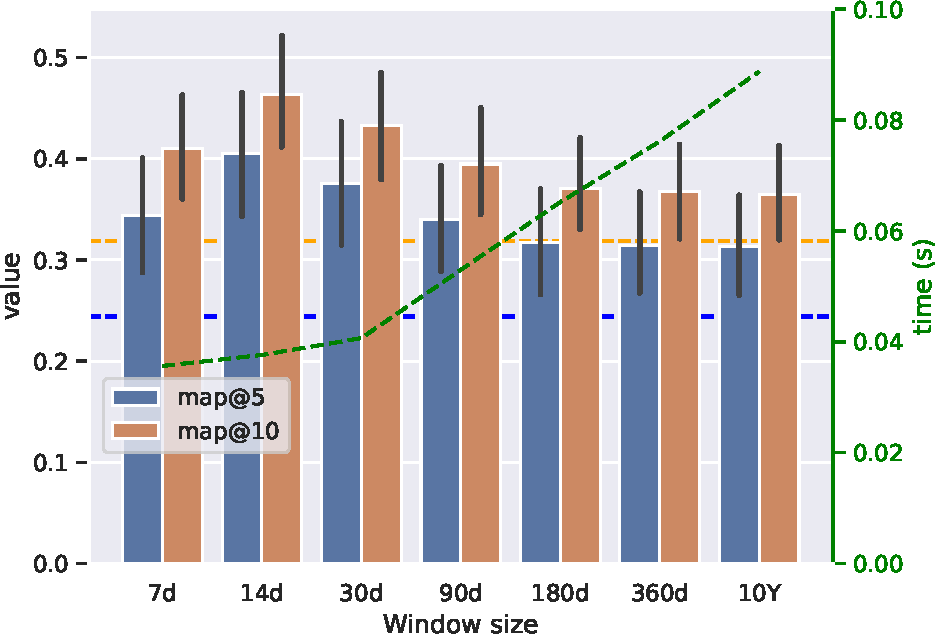
\includegraphics[height=45mm]{./images/graphs/11_cosine_results_window-size_W-THU_normalize=True.pdf}
        \caption{Rendimiento del modelo PLN con respecto al tamaño de la ventana de entrenamiento}
    \end{figure}
\end{frame}

\subsection{Modelo basado en filtrado colaborativo}
\begin{frame}{LightGCN}
    % TODO: ¿Pongo la formula de los embeddings y la agregación? Yo creo que sí, la figura del paper también tá chula.
    \footnotesize
    \vspace{-3pt}
    \begin{columns}
        \column{.5\linewidth}
        \begin{figure}
            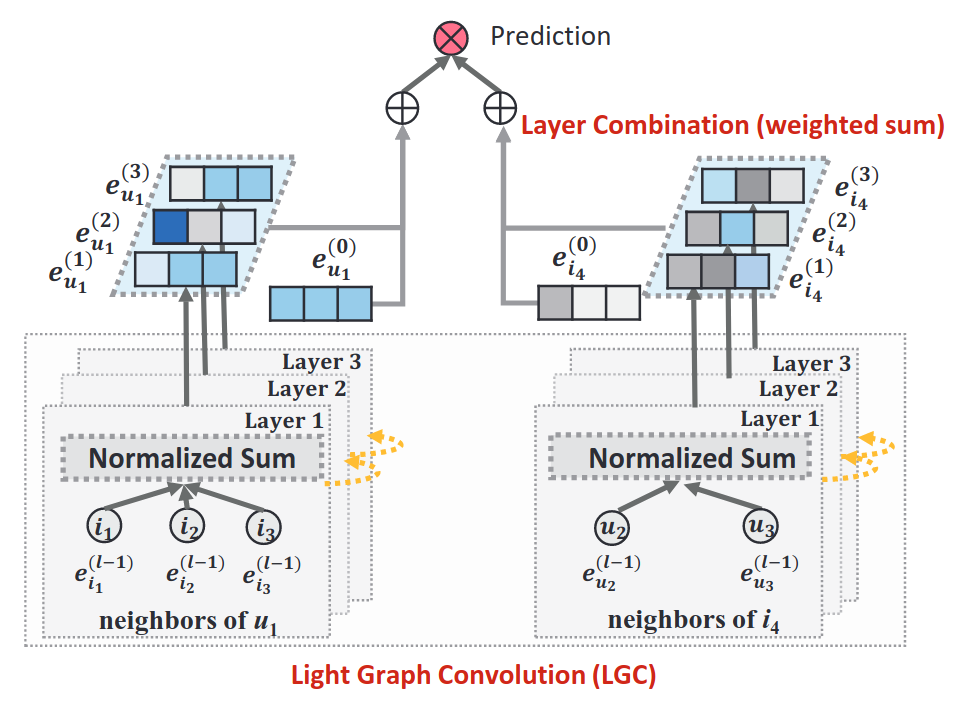
\includegraphics[width=.95\linewidth]{./images/screenshots/lightgcn_fig2.png}
        \end{figure}
        \column{.5\linewidth}
        \begin{exampleblock}{Light Graph Convolution}
            \vspace{-2pt}
            $$ 
            {\color{DarkOrange}e_u^{(k+1)}} = 
            \sum_{i\in \mathcal{N}} \frac{1}{
                \sqrt{\left|\mathcal{N}_u\right|}
                \sqrt{\left|\mathcal{N}_i\right|}
            }
            {\color{RoyalBlue}e_{i}^{(k)}}
            $$
            \vspace{-2pt}
        \end{exampleblock}
        \pause
        \begin{exampleblock}{Embedding final}
            \vspace{-2pt}
            $$ 
            {\color{DarkOrange}e_u} = \sum_{k=0}^K {\color{DarkOrange}e_u^{(k)}};\;
            {\color{RoyalBlue}e_i} = \sum_{k=0}^K {\color{RoyalBlue}e_i^{(k)}}
            $$
            \vspace{-2pt}
        \end{exampleblock}
    \end{columns}
    \blfootnote{\footcite{he_lightgcn_2020}}
\end{frame}

\begin{frame}{Fine-tuning de LightGCN I}
\begin{table}[]
    \centering
    \begin{tabular}{l|c|c}
\textbf{Hiperparámetro} & \textbf{Valores} & \textbf{Muestreo} \\
\hline
Embedding dim. & $1\leq e\leq 1024, e\in \mathbb{N}$ & Loguniforme \\
Convolution layers & $c\in \{1,2,3,4,5,6\}$ & Uniforme \\
Batch size & $bs\in\{64,128,256,512,1024\}$ & Uniforme \\
Learning rate & $10^{-4}\leq lr\leq 1, lr\in \mathbb{R}$ & Loguniforme \\
L2 regularization & $10^{-7}\leq l2 \leq 10^{-2}, l2 \in \mathbb{R}$ & Loguniforme \\
    \end{tabular}
    \caption{Espacio de búsqueda de hiperparámetros para LightGCN}
\end{table}
\blfootnote{\footcite{bergstra_making_2013}}
\blfootnote{\footcite{liaw_tune_2018}}
\end{frame}

\begin{frame}{Fine-tuning de LightGCN II}
    % Aquí pondre como una especie de ``progress bar" que se rellene con distintos colores para indicar la parte que se usa para elegir los hiperparámetros y la que se testea como ``modelo realista''
    \begin{figure}
        \centering
        \begin{tikzpicture}
            \def\trainw{3.3cm}
            \def\testw{.7cm}
            \def\recth{0.5cm}
            \def\rectspace{0.25cm}

            % Draw the four main rectangles (train and test)
            \pgfmathsetlengthmacro{\lastybot}{-4*(\recth+\rectspace)}
            \pgfmathsetlengthmacro{\bestybot}{-1*(\recth+\rectspace)}
            \foreach \i/\v in {0/0.21,1/0.34,2/0.25,3/0.17} {
                \pgfmathsetlengthmacro{\ybot}{(-\i*(\recth + \rectspace))}
                \pgfmathsetlengthmacro{\ytop}{\ybot-\recth}

                \draw[
                    thick,
                    fill=Green!20,
                    draw=Green
                ]
                    (0,\ybot)
                    rectangle
                    (\trainw,\ytop);
                \node[anchor=east] at (0,\ybot-\recth/2) {$H_\i$};
                \draw[
                    thick,
                    fill=RoyalBlue!20,
                    draw=RoyalBlue,
                ] 
                (\trainw,\ybot)
                rectangle
                (\trainw+\testw,\ytop)
                node[midway,right=3mm] (val\i) {\v};
            }

            % Draw the braces
            \draw[
                decorate,
                decoration={brace,amplitude=10pt,raise=5pt},
            ]
            (0,0) -- (\trainw,0)
            node[anchor=south,midway,above=15pt] {Entrenamiento};
            \draw[
                decorate,
                decoration={brace,amplitude=10pt,mirror},
            ]
            (0,\lastybot) -- (\trainw+\testw,\lastybot)
            node[anchor=north,midway,below=7pt] {Fold $n$};

            \pause
            % Draw the arrow
            \draw[
                -stealth,
            ] (val2.east) to ++(10mm,0) node [right] (nextfold) {$H_2$};

            % Draw the right rectangle
            \draw[
                thick,
                fill=Green!20,
                draw=Green,
            ]
            (nextfold.south east) rectangle ++(\trainw+1cm,\recth) node (nextfoldt) {};
            \draw[
                thick,
                fill=RoyalBlue!20,
                draw=RoyalBlue,
            ] (nextfoldt) rectangle ++(\testw,-\recth) node (nextfoldf) {};

            % Draw the next brace
            \draw[
                decorate,
                decoration={brace,amplitude=10pt,mirror},
            ]
            ($(nextfold.south east)+(0,-\rectspace)$) -- ($(nextfoldf)+(0,-\rectspace)$)
            node[anchor=north,midway,below=7pt] {Fold $n+1$};

            % Force "finishing" the picture even on the first slide
            % https://tex.stackexchange.com/a/70051/107093
            \onslide<1->
        \end{tikzpicture}
    \end{figure}
\end{frame}

\begin{frame}{Resultados GNN}
\begin{columns}
\column{.5\linewidth}
\begin{figure}
    \centering
    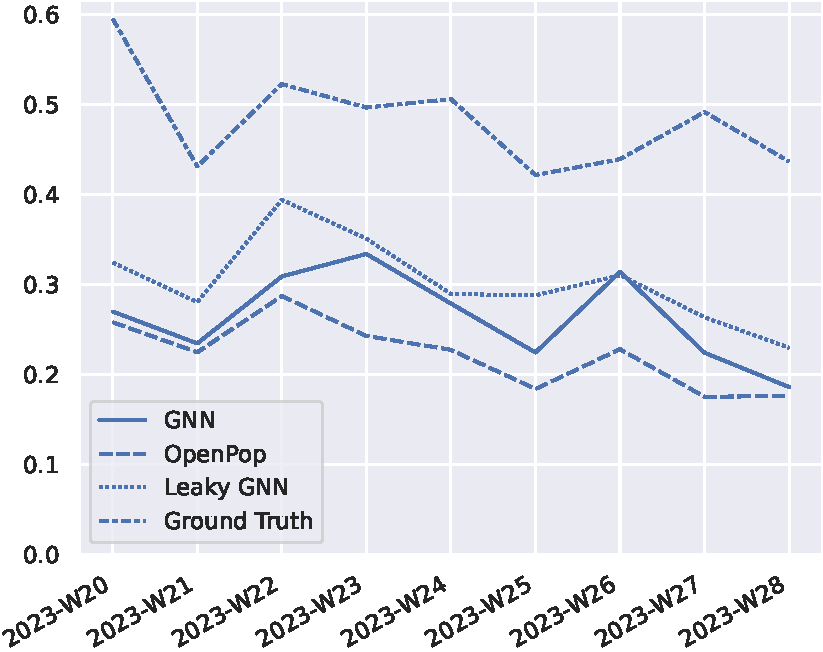
\includegraphics[height=45mm]{./images/graphs/09_gnn_results_precision_5_leaky.pdf}
    \caption{precision@5 del modelo GNN}
\end{figure}
\column{.5\linewidth}
\begin{figure}
    \centering
    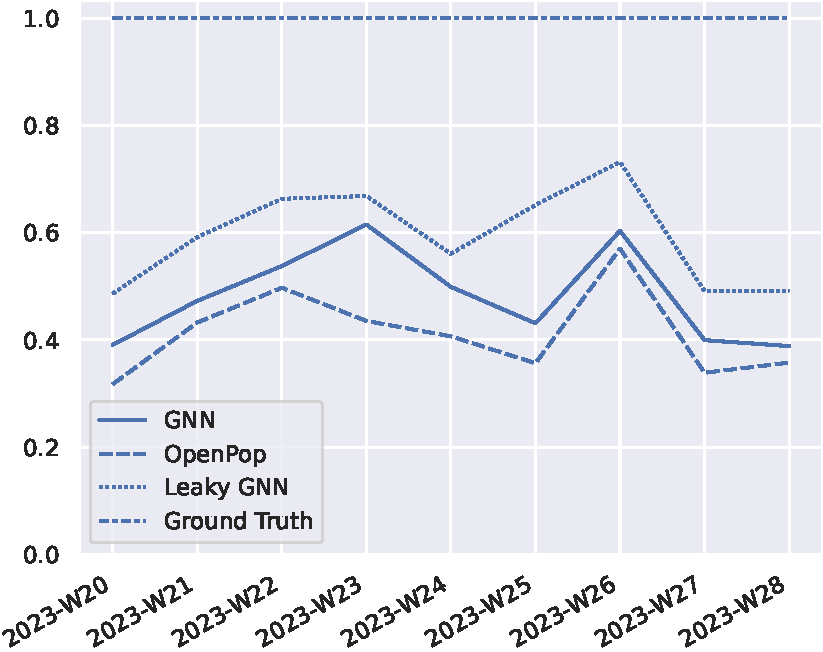
\includegraphics[height=45mm]{./images/graphs/09_gnn_results_ndcg_10_leaky.pdf}
    \caption{ndcg@10 del modelo GNN}
\end{figure}
\end{columns}
\end{frame}

\subsection{Modelo híbrido}
\begin{frame}{Comparación recomendaciones}
    \begin{figure}
        \centering
        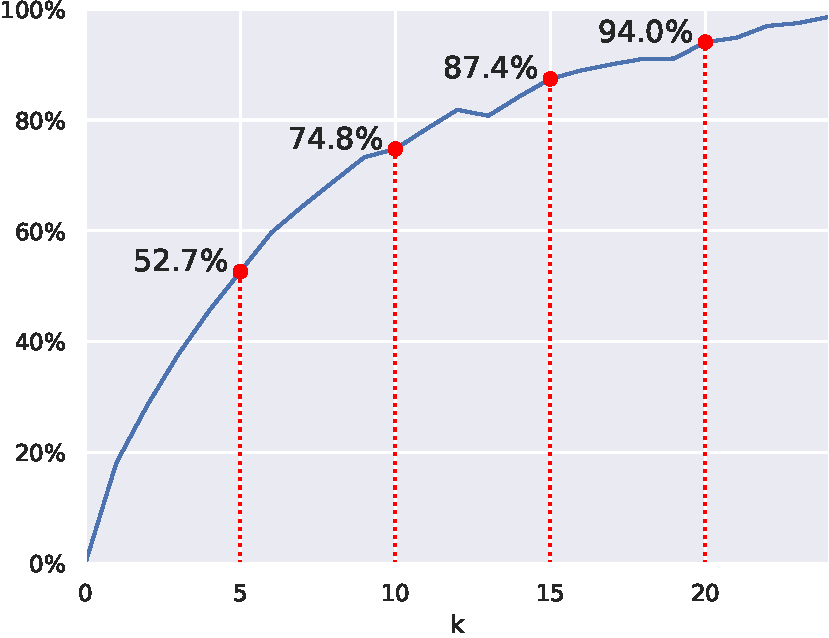
\includegraphics[height=45mm]{./images/graphs/12_hybrid_common_Decentraland_W-THU_normalize=True.pdf}
        \caption{Porcentaje de propuestas en común entre los dos recomendadores}
    \end{figure}
\end{frame}    

\begin{frame}{Métodos de fusión}
    \begin{figure}
        \centering
        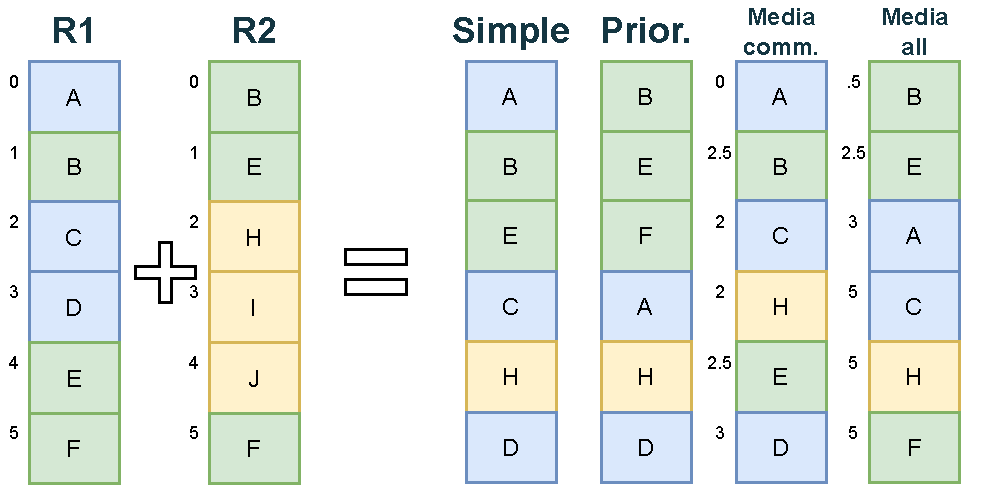
\includegraphics[height=45mm]{./images/diagrams/metodos-fusion.drawio.pdf}
        \caption{Distintos métodos de fusión utilizados}
    \end{figure}
\end{frame}

\begin{frame}{Resultados}
    \begin{figure}
        \centering
        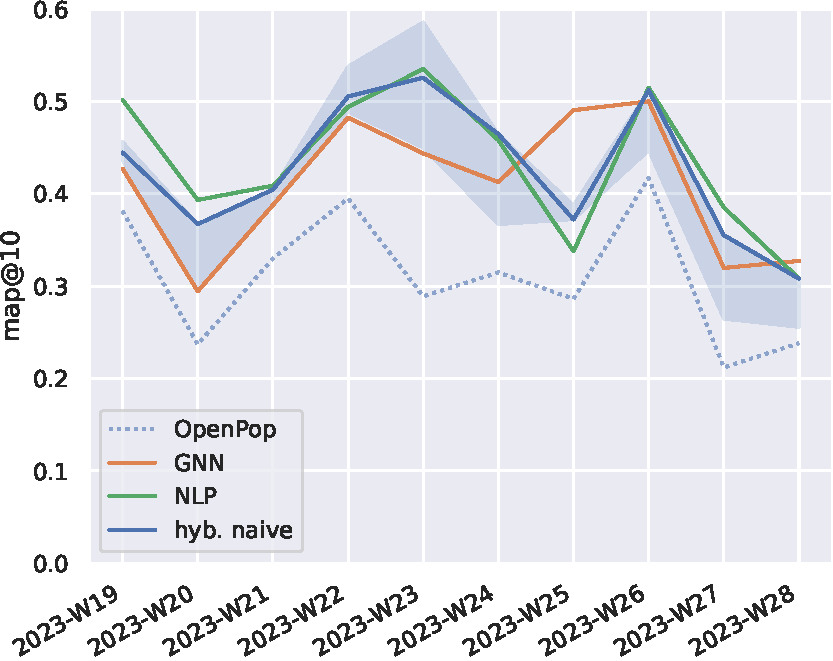
\includegraphics[height=45mm]{./images/graphs/12_hybrid_merge_results_folds_Decentraland_W-THU_normalize=True_compare.pdf}
        \caption{Resultados en cada fold de los sistemas recomendadores}
    \end{figure}
\end{frame}